\begin{frame}
\frametitle{Evaluación}

\begin{itemize}
	\item<1-> Se han procedido a realizar diferentes pruebas con distintas variables.
	
	\vspace{1em}
	
	\item<2-> Por ejemplo, definiendo distintos tamaños de escenarios.
	
	\vspace{1em}
	
	\item<3-> El tiempo de ejecución aumenta \textcolor{UDCpink}{exponencialmente}.
\end{itemize}

\vspace{1em}

\pause[3]

\centering
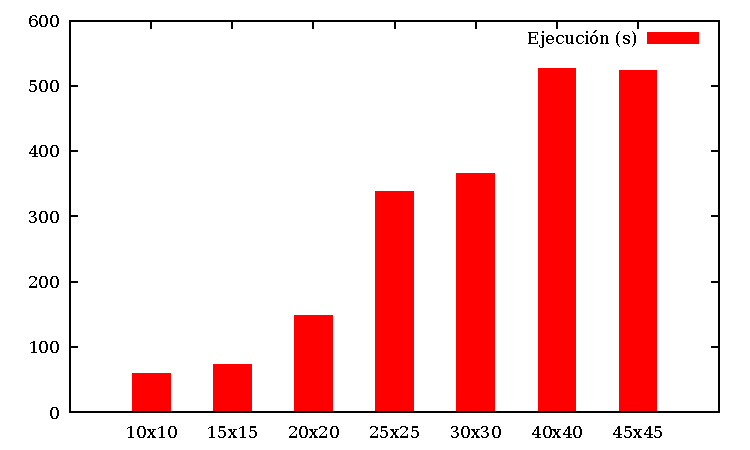
\includegraphics[width=0.6\textwidth]{images/map-size.pdf}

\end{frame}

\begin{frame}
\frametitle{Evaluación}

\begin{itemize}
	\item<1-> Modificado porcentajes de terreno con tierra y tamaño de biomas.
	
	\vspace{0.5em}
	
	\item<2-> Se observa la \textcolor{UDCpink}{tendencia exponencial} como en la primera prueba.
\end{itemize}

\pause[2]

\begin{table}[!h]
	\centering
	\begin{tabular}{c|cccccc}
		& 10\% & 15\% & 20\% & 25\% & 30\% & 35\% \\
		\hline
		10\% & 42 & 41 & 35 & 88 & 117 & 214 \\
		15\% & 41 & 37 & 36 & 88 & 133 & 247 \\
		20\% & 37 & 43 & 37 & 105 & 123 & 224 \\
		25\% & 29 & 51 & 43 & 92 & 123 & 220 \\
		30\% & 42 & 43 & 138 & 95 & - & - \\
		35\% & 41 & 40 & 38 & 90 & - & 241 \\
		40\% & 43 & 46 & 36 & -  & - & 217  \\
		45\% & 69 & 49 & 36 & 737 & - & 220 \\
		50\% & 100 & - & 1064 & - & - & - \\
		55\% & 55 & 956 & - & - & - & - \\
		60\% & 164 & 740 & - & - & - & - \\
		65\% & 97 & 838 & - & - & - & - \\
		\hline
	\end{tabular}
\end{table}

\end{frame}